\documentclass[11pt]{article}
\usepackage[margin=1in]{geometry}
\usepackage{amsmath,amssymb,amsthm}
\usepackage{graphicx}
\usepackage[hidelinks]{hyperref}

\newtheorem{theorem}{Theorem}
\newtheorem{lemma}{Lemma}
\newcommand{\N}{\mathbb N}
\newcommand{\ellTwo}{\ell_2(\N)}
\newcommand{\Tr}{\operatorname{Tr}}

\title{A Bounded Perturbation Which Spoils a Heat-Trace Expansion}
\author{run fa\_banach\_001, lane 15}
\date{2026-07-18}

\begin{document}
\maketitle

\section*{Source Signal}

Eckstein--Zajac, arXiv:1412.5100, study asymptotic and exact expansions of
heat traces for positive unbounded operators with compact inverses.  In their
concluding discussion, p. 38, they point to the behavior of the heat trace
under bounded perturbations as a natural next step: a bounded perturbation does
not change the leading small-time behavior, but may spoil the full asymptotic
expansion.

\begin{center}
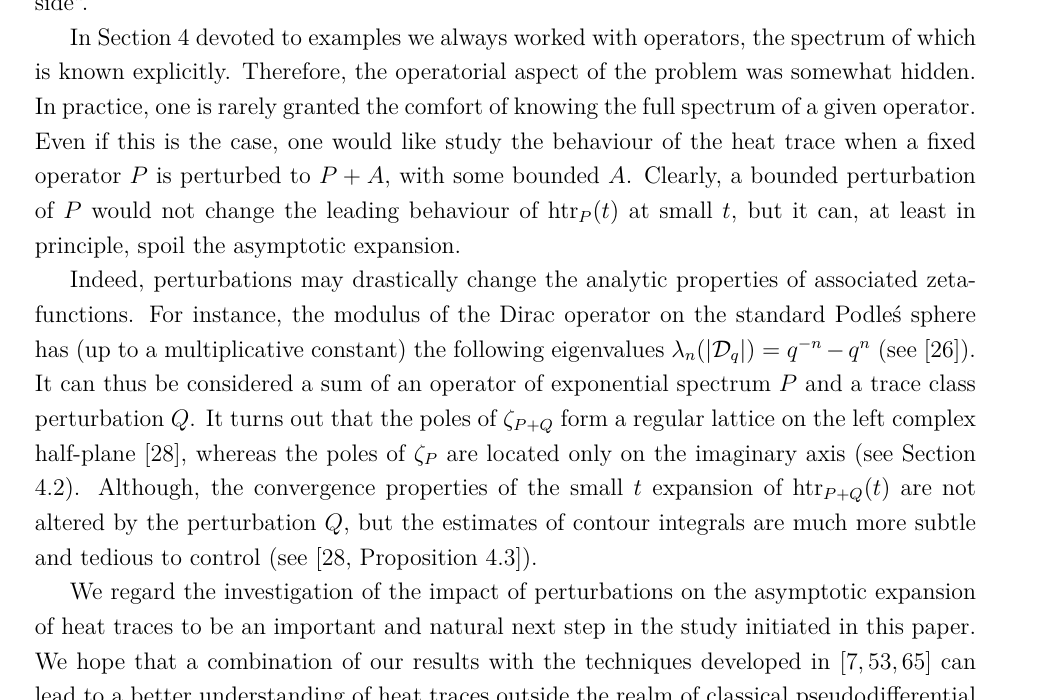
\includegraphics[width=0.92\linewidth]{figures/source_perturbation_question_crop.png}
\end{center}

\section*{Result}

\begin{theorem}
There are a positive self-adjoint compact-resolvent operator $P_0$ on
$\ellTwo$ and a bounded positive self-adjoint diagonal operator $A$ with
$0\leq A\leq I$ such that:
\begin{enumerate}
\item $\Tr(e^{-tP_0})$ has an exact Laurent expansion at $t=0$;
\item $P=P_0+A$ still satisfies $\Tr(e^{-tP})\sim t^{-1}$ as $t\downarrow0$;
\item there is no constant $c$ such that
\[
  \Tr(e^{-tP})=t^{-1}+c+o(1).
\]
\end{enumerate}
Thus an arbitrary bounded perturbation can destroy the heat-trace expansion
already at the constant term.
\end{theorem}

\section*{Proof Intuition}

For $P_0 e_n=n e_n$, the heat trace is the geometric series
$(e^t-1)^{-1}$.  A diagonal $0/1$ perturbation changes only selected
eigenvalues, replacing $e^{-tn}$ by $e^{-t(n+1)}$ on a set $S\subset\N$.
The error is therefore $(e^{-t}-1)\sum_{n\in S}e^{-tn}$.  If $S$ has no Abel
density, this error has no limit at order $t^0$.

\section*{Proof}

Let $H=\ellTwo$ with standard unit vector basis $(e_n)_{n\geq1}$ and set
\[
  P_0 e_n = n e_n .
\]
Then $P_0$ is positive, self-adjoint, and has compact inverse.  Its heat trace
is
\[
  H_0(t)=\Tr(e^{-tP_0})=\sum_{n=1}^{\infty}e^{-tn}
       =\frac{1}{e^t-1}
       =t^{-1}-\frac12+O(t).
\]

Choose integers $N_1<N_2<\cdots$ such that $N_{k+1}/N_k\to\infty$; for
example, $N_1=2$ and $N_{k+1}=N_k^2$.  Put
\[
  S=\bigcup_{m\geq1}\{N_{2m},N_{2m}+1,\ldots,N_{2m+1}-1\}.
\]
Define the bounded diagonal operator $A$ by
\[
  A e_n=\mathbf 1_S(n)e_n .
\]
Then $0\leq A\leq I$, and $P=P_0+A$ is again positive self-adjoint with
compact inverse.  Write
\[
  F(t)=\sum_{n\in S}e^{-tn}.
\]
Since the spectra are diagonal,
\[
  H(t):=\Tr(e^{-tP})
  =\sum_{n\notin S}e^{-tn}+\sum_{n\in S}e^{-t(n+1)}
  =H_0(t)+(e^{-t}-1)F(t).
\]
Because $0\leq F(t)\leq H_0(t)$, the perturbation term is $O(1)$, hence
$tH(t)\to1$.

We now show that the constant term cannot exist.  Let
$t_m=N_{2m+1}^{-1}$.  The contribution of the occupied block
$[N_{2m},N_{2m+1})$ gives a Riemann sum:
\[
  t_m\sum_{n=N_{2m}}^{N_{2m+1}-1} e^{-t_m n}
  \longrightarrow \int_0^1 e^{-x}\,dx
  =1-e^{-1}.
\]
The earlier blocks contribute at most $t_m N_{2m-1}\to0$, and the later blocks
contribute at most a geometric tail beginning at $N_{2m+2}$, which is
$o(1)$ after multiplication by $t_m$.  Therefore
\[
  t_m F(t_m)\longrightarrow 1-e^{-1}.
\]

Next choose $M_m=\lfloor (N_{2m+1}N_{2m+2})^{1/2}\rfloor$ and
$u_m=M_m^{-1}$.  The point $M_m$ lies deep in the empty gap after
$N_{2m+1}$.  All earlier occupied blocks contribute at most
$u_m N_{2m+1}\to0$, while all later occupied blocks begin after
$N_{2m+2}$ and contribute $o(1)$ after multiplication by $u_m$.  Hence
\[
  u_m F(u_m)\longrightarrow0.
\]

Finally, since $e^{-t}-1=-t+O(t^2)$ and $F(t)\leq H_0(t)=O(t^{-1})$,
\[
  (e^{-t}-1)F(t)=-tF(t)+o(1).
\]
Thus
\[
  H(t_m)-t_m^{-1}\longrightarrow -\frac12-(1-e^{-1}),
\]
whereas
\[
  H(u_m)-u_m^{-1}\longrightarrow -\frac12.
\]
The quantity $H(t)-t^{-1}$ has two different subsequential limits as
$t\downarrow0$.  Consequently no constant $c$ can satisfy
$H(t)=t^{-1}+c+o(1)$, and the heat trace of $P_0+A$ has no classical
asymptotic expansion beyond the leading term.

\section*{Verification And Scope}

The perturbation is bounded, positive, self-adjoint, and diagonal, but it is
not compact.  The result therefore addresses arbitrary bounded perturbations
of compact-resolvent Hilbert-space operators.  It does not contradict
structured preservation theorems for elliptic, pseudodifferential,
trace-class, or regular spectral-triple perturbations.

Local index search found no exact prior row for arXiv:1412.5100.  Web searches
for bounded perturbations of heat-trace asymptotics found preservation
statements in structured settings but no exact diagonal counterexample of the
form above.

\section*{References}

\begin{itemize}
\item M. Eckstein and A. Zajac, ``Asymptotic and exact expansions of heat
traces'', arXiv:1412.5100; Math. Phys. Anal. Geom. 18 (2015), article 28.
\end{itemize}

\end{document}
